%
% emwelle.tex -- template for standalon tikz images
%
% (c) 2024 S. Oseghale, M. Doswald
%
\documentclass[tikz]{standalone}
\usepackage{amsmath}
\usepackage{times}
\usepackage{txfonts}
\usepackage{pgfplots}
\usepackage{csvsimple}
\colorlet{myblue}{black!40!blue}
\colorlet{myred}{black!40!red}
\colorlet{vcol}{green!50!black}
\colorlet{Ecol}{orange!90!black}
\colorlet{EVcol}{orange!80!black!60}
\colorlet{Bcol}{violet!90}
\usetikzlibrary{arrows,intersections,math}
\begin{document}
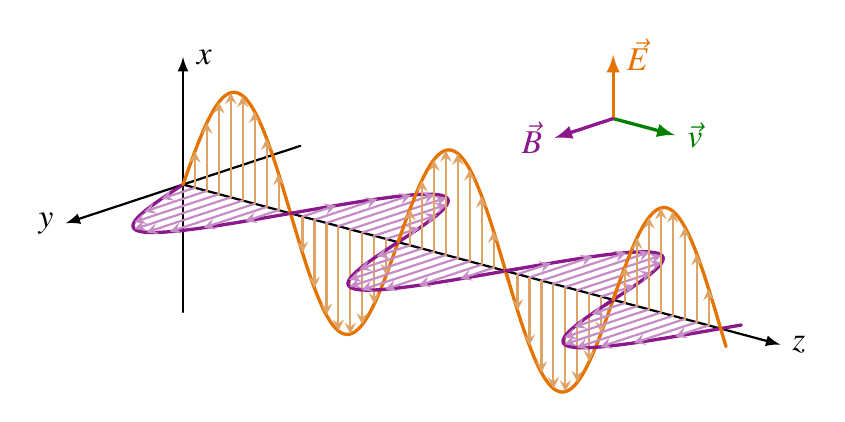
\begin{tikzpicture}[>=latex,thick,
	x=(-15:0.9), y=(90:0.9), z=(-150:1.1),
	line cap=round, line join=round,
	axis/.style={black, thick,->},
	vector/.style={>=stealth,->}]
	\large
	\def\A{1.5}
	\def\nNodes{5} % use even number
	\def\nVectorsPerNode{8}
	\def\N{\nNodes*40}
	\def\xmax{\nNodes*pi/2*1.01}
	\pgfmathsetmacro\nVectors{(\nVectorsPerNode+1)*\nNodes}
	\def\vE{{\color{Ecol}\mathbf{E}}}
	\def\vB{{\color{Bcol}\mathbf{B}}}
	
	\def\drawENode{ % draw E node and vectors with some offset
		\draw[Ecol,very thick,variable=\t,domain=\iOffset*pi/2:(\iOffset+1)*pi/2*1.01,samples=40]
		plot (\t,{\A*sin(\t*360/pi)},0);
		\foreach \k [evaluate={\t=\k*pi/2/(\nVectorsPerNode+1);
			\angle=\k*90/(\nVectorsPerNode+1);}]
		in {1,...,\nVectorsPerNode}{
			\draw[vector,EVcol]  (\iOffset*pi/2+\t,0,0) -- ++(0,{\A*sin(2*\angle+\iOffset*180)},0);
		}
	}
	\def\drawBNode{ % draw B node and vectors with some offset
		\draw[Bcol,very thick,variable=\t,domain=\iOffset*pi/2:(\iOffset+1)*pi/2*1.01,samples=40]
		plot (\t,0,{\A*sin(\t*360/pi)});
		\foreach \k [evaluate={\t=\k*pi/2/(\nVectorsPerNode+1);
			\angle=\k*90/(\nVectorsPerNode+1);}]
		in {1,...,\nVectorsPerNode}{
			\draw[vector,Bcol!50]  (\iOffset*pi/2+\t,0,0) -- ++(0,0,{\A*sin(2*\angle+\iOffset*180)});
		}
	}
	
	% MAIN AXES
	\draw[axis] (0,0,0) -- ++(\xmax*1.1,0,0) node[right] {$z$};
	\draw[axis] (0,-\A*1.2,0) -- (0,\A*1.2,0) node[right] {$x$};
	\draw[axis] (0,0,-\A*1.2) -- (0,0,\A*1.2) node[left] {$y$};
	
	% SMALL AXES
	\def\xOffset{{(\nNodes-2)*pi/2}}
	\def\yOffset{\A*1.1}
	\def\zOffset{\A*1.1}
	\draw[axis,very thick,vcol] (\xOffset,\yOffset,-\zOffset) -- ++(\A*0.6,0,0) node[right,align=center] {$\vec{v}$}; %\\propagation
	\draw[axis,very thick,Ecol]  (\xOffset,\yOffset,-\zOffset) -- ++(0,\A*0.6,0) node[right] {$\vec{E}$};
	\draw[axis,very thick,Bcol]   (\xOffset,\yOffset,-\zOffset) -- ++(0,0,\A*0.6) node[left] {$\vec{B}$};
	
	% draw (anti-)nodes
	\foreach \iNode [evaluate={\iOffset=\iNode-1;}] in {1,...,\nNodes}{
		\ifodd\iNode \drawBNode \drawENode % E overlaps B
		\else        \drawENode \drawBNode % B overlaps E
		\fi
	}
\end{tikzpicture}
\end{document}
